\chapter{Background}\label{chap:Background}


\section{GPU Overview}\label{GPU-info}
% This section provides a brief overview of GPGPU and CUDA.
\subsection{History and Motivation}\label{sec:History}
In the world of computational hardware, microprocessors based on single processing cores (traditional CPUs) have driven rapid performance improvements in floating-point operations per second (FLOPS) for nearly 2 decades $(1985-2003)$.
These microprocessors were capable of performing in the range of Giga-FLOPS $(10^9)$ on desktops and Tera-FLOPS $(10^{12})$ on data centers \cite{GPU_book_wen-mei}.
This improvement drive flattened due to fundamental problems such as thermal stability, energy density, and quantum effects.
Since then, all microprocessors have adapted architectures with multiple processing cores and thread virtualization to keep up with the improvements expected by the market. Naturally, it needed significant change in software to keep up with the reported performance and increasing computational requirements \cite{Sutter-multi-core-programming}.

High-Definition Graphics demand from the gaming industry was one of the biggest drivers for such high-performance hardware. The performance demanded here is throughput oriented, i.e., generating maximum frames per second while the computational requirement for each pixel is sufficiently low.
Some chip manufacturers like NVIDIA took a different approach of multi-thread hardware  to cater to these requirements \cite{GPUs_and_gaming}.
The hardware designed with this philosophy had threads capable of performing simple computational tasks with relatively lower clock speed to give an overall performance in Tera-FLOPS range. On top of that, the hardware gave more performance per watt which made it possible to add to a desktop machine \cite{ppw_gpu_vs_cpu}.
Modern GPUs have also proven to be fast and cost-effective for deep learning and image processing tasks contributing to many advances in fields like computer vision and artificial intelligence. A modern data center GPU, for example (NVIDIA A100), now has more than 100,000 concurrent threads. These threads execute in many simple pipelines to give around 10 times faster raw performance than state-of-the-art CPUs \cite{GPU_book_wen-mei}.
\begin{figure}
    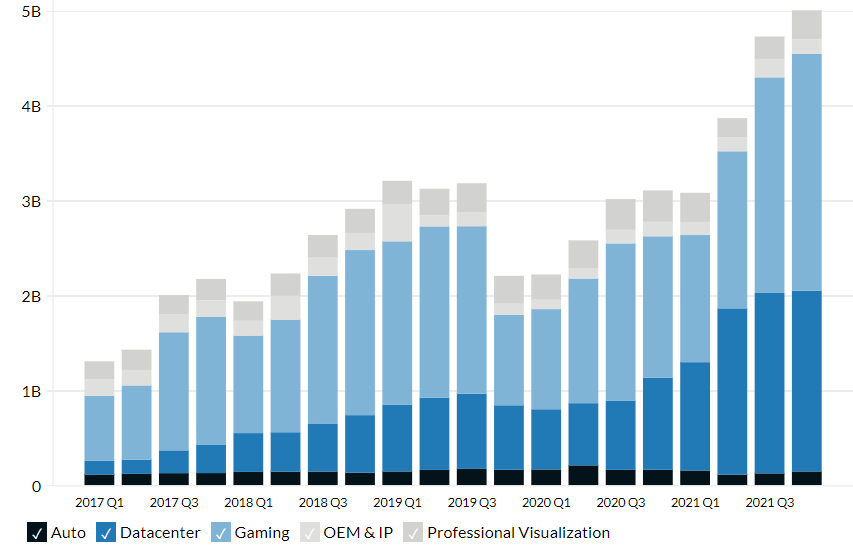
\includegraphics[width=\textwidth]{fig/Nvidia-revenue-by-end-market.png}
    \source{Business Quant \cite{business-quant}}
    \caption{Nvidia Revenue by End Market}
    \label{fig:Nvidia-revenue}
\end{figure}

Figure \ref{fig:Nvidia-revenue} shows that Nvidia GPU data center market has improved significantly in recent years to become almost equivalent to the already huge gaming industry.
This has fueled the hardware and software development of current server-grade GPUs which has enabled huge computational potential for deep learning.
While HPC hardware improves at such rapid pace, software solutions for graph theory problems still need to move from \textit{multi core} paradigm to \textit{multi thread}.

\subsection{Heterogeneous Programming Environment}
\begin{figure}[ht]
    \begin{minipage}{0.35\textwidth}
        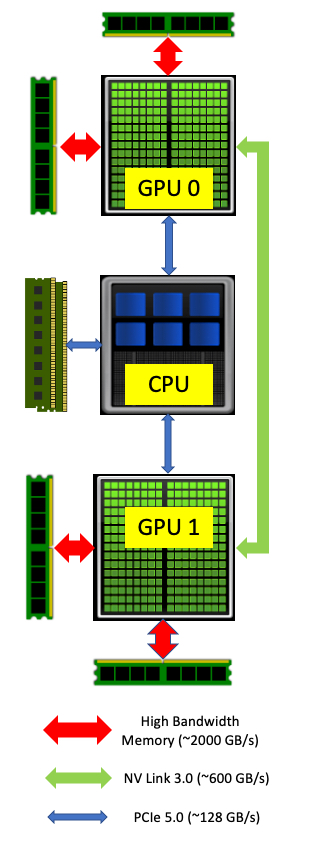
\includegraphics[width=\textwidth]{fig/cpu-gpu-arch.jpg}
    \end{minipage}
    \begin{minipage}{0.6\textwidth}
        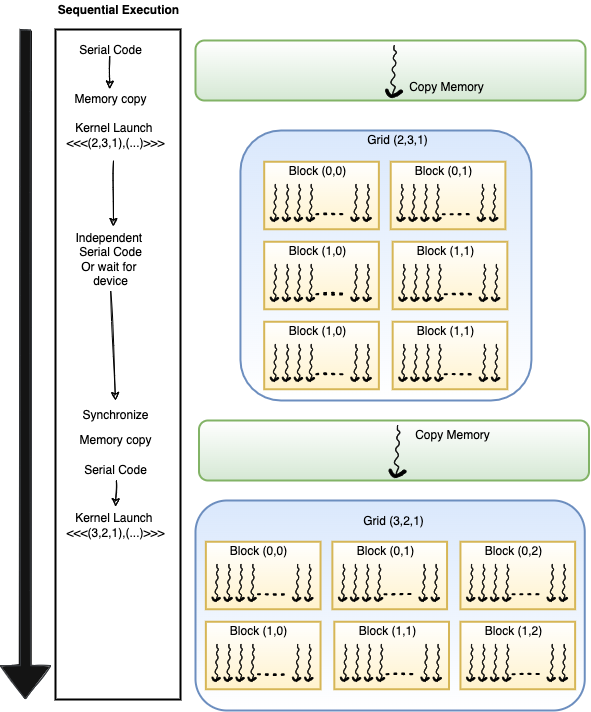
\includegraphics[width=\textwidth]{fig/heterogeneous-programming.png}
    \end{minipage}
    \caption{CUDA Heterogeneous Programming Model}
    \label{fig:Heterogenous-Programming}
\end{figure}
GPU is a throughput oriented computational hardware.
A single thread of a GPU is significantly slower than a CPU. Hence, working with it for inherently sequential tasks can incur huge latencies.
Since many basic programming tasks are inherently sequential and the whole operating system environment is developed for latency optimized processors (CPUs), GPUs work better off being used as a supplemental piece of hardware along with CPUs for computationally intensive tasks.
Hence, GPUs are mostly used in a Heterogeneous programming environment with CPU (host) executing the governing code while offloading computationally intensive tasks as kernels to GPUs (device).
Note that one host can be connected to multiple devices.
Since the memory of device and host are different, the input and output data need to be copied before and after kernel execution.
Figure \ref{fig:Heterogenous-Programming} shows the high level hardware and software architecture.
GPUs can communicate with CPU via PCIe (Peripheral Component Interconnect express) bus and with each other via NVLink \texttrademark.
The memory bandwidth of PCIe is the lowest and hence it is in best interests to avoid high data transfers between GPU and CPU.
Native memory of the GPU or the VRAM, is High Bandwidth Memory (HBM) with the latest generation having bandwidth of around 2000 GB/sec.
The Nvidia proprietary GPU Interconnect with 12 links per GPU can provide up to 600 GB/sec.
While the industry standard PCIe bus gen 5.0 with 32 links can provide up to 128 GB/sec of bandwidth.

\subsection{Thread Hierarchy}\label{sec:thread-hierarchy}
As discussed in Section \ref{sec:History} GPUs have \textit{multi thread} architecture with hundreds of thousands of threads. To have such massive hardware parallelism threads have to collaborate on usage of different resources for ex.\textit{cuda cores}.
%
Since all threads do not share these resources, it is important to understand thread Hierarchy in GPUs.

\begin{figure}[h]
    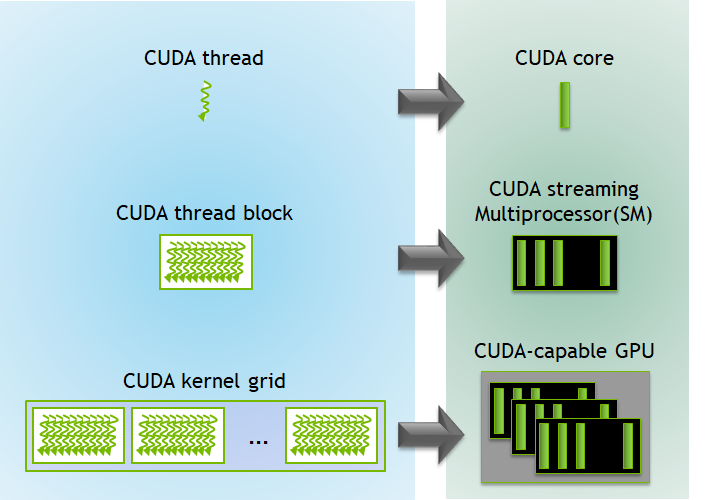
\includegraphics[width=\textwidth]{fig/thread-hierarchy.png}
    \source{Nvidia Developer Blog \cite{developer-blog}}
    \caption{Thread Hierarchy}
    \label{fig:Thread-Hierarchy}
\end{figure}

A thread is a single sequential flow of control within a program.
A block is a chunk of threads while a grid is a chunk of blocks.
Since threads are virtual they need to be optimally assigned hardware resources to perform tasks.
Figure \ref{fig:Thread-Hierarchy} shows how these virtual entities are mapped to the hardware. As discussed a thread utilizes a \textit{cuda core} for performing computation. A block of threads resides on a \textit{Streaming Multiprocessor} (SM), which is a hardware block that consists of computational resources like \textit{cuda cores, memory controllers, tensor cores}, etc. Thread block resides on an SM for the entirety of its execution. Hence, multiple threads in a block can utilize the same core. Multiple blocks can reside on an SM simultaneously within limits.
GPU has multiple SMs and hence many blocks can concurrently reside on the GPU during a context. If a grid requests more blocks than that can concurrently reside on the GPU, their execution is serialized.
Nvidia's latest server-grade GPU A100 has 108 SMs with a maximum of 32 blocks or 2048 threads residing per SM which means the maximum number of concurrent threads is  221,184. While on the hardware side, A100 has 6912 \textit{cuda cores}, i.e., 64 cores per SM. So, during execution, all 2048 threads in a block will compete for these 64 cores.

To add further, the thread instructions are processed in a Single Instruction Multi Data (SIMD) model. This SIMD chunk of threads is allocated resources at once, this chunk is called \textit{warp}. If threads within a warp demand different operations then all threads within that warp perform all operations with output of undesired threads being ignored. This causes a slowdown in execution and is referred as \textit{warp divergence}. Hence, algorithms and implementations need to be designed in such a way that \textit{warp divergence} is minimized. While the size of thread block and grid are configurable by the programmer, warp size is a fixed architectural parameter.

\begin{figure}[h]
    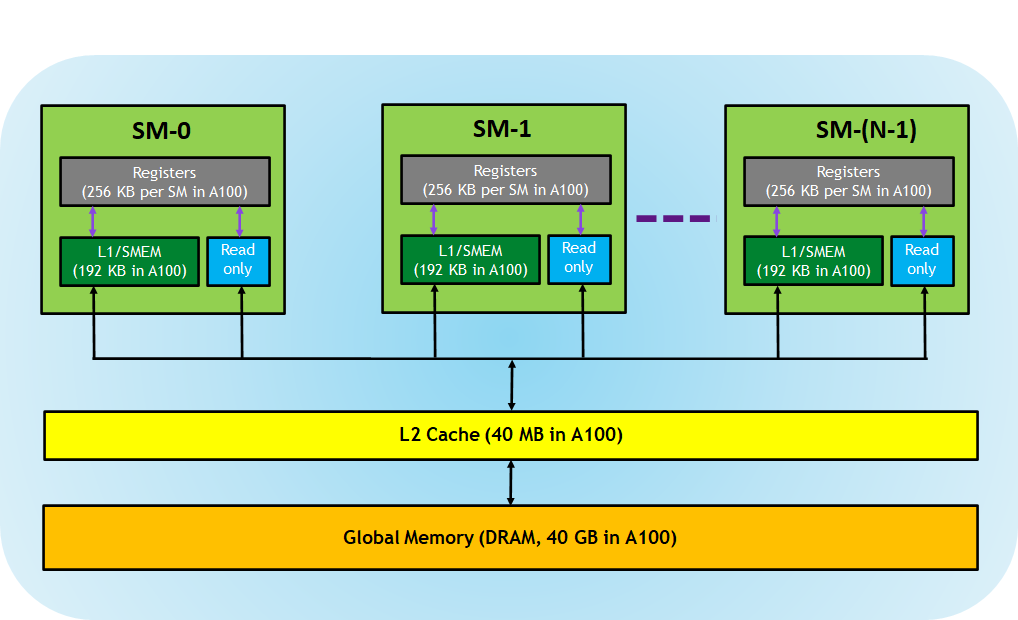
\includegraphics[width=\textwidth]{fig/memory-hierarchy.png}
    \source{Nvidia Developer Blog \cite{developer-blog}}
    \caption{GPU Memory Hierarchy}
    \label{fig:Memory-Hierarchy}
\end{figure}

\subsection{Memory Hierarchy}
GPU needs high performance memory system as it can be easily stressed due to the underlying massive parallelism.
If the available memory bandwidth is overwhelmed, threads need to wait for data to be able to perform computation even though some processing cores are free. This results in poor utilization and overall slower performance.
Even though GPU memory is significantly faster than conventional RAM, it can still limit application performance.
This problem is alleviated by building memory caches on the chip die itself, so accessing them is significantly faster (around 100 - 1000 times) but they have size restrictions.
Modern compilers identify repeated memory accesses and can aggressively cache to reduce memory stress.
The memory bandwidth problem is not significant for CPUs as they have huge cache banks per thread core. But for GPUs the cache per thread (L1 cache) is very restrictive.

GPU memory architects have tried to solve this problem by adding hierarchical memory banks. There are 3 types of memory banks on a GPU namely \textit{Global}, \textit{Shared} and \textit{Register} memory.
Figure \ref{fig:Memory-Hierarchy} shows the memory hierarchy, as name suggests global memory is accessible by all threads, it is equivalent to the Random Access Memory (RAM) on CPUs and is also sometimes referred as Video RAM (VRAM) or Device RAM (DRAM).
Shared memory is accessible by all threads in a thread block.
Register memory is private to each thread.
The size limitations on these memory banks are based on SM architecture and hardware.
Programmers are also equipped with read-only constant memory (not shown in the Figure) which is accessible by all threads.
Unknown to the programmer, compilers can also utilize these memory banks by caching in register and shared memory banks if repeated accesses to global memory are detected. It is referred as L1 cache. Equivalent to CPU cache there is also an L2 cache for use by the compiler only and accessible to all threads.

As discussed, memory utilization plays a significant role in code performance, a program whose execution time is restricted by memory is called memory bound. Memory bound programs do not scale well with increasing number of devices as distributing computation to other workers does no benefit and further increases latency due to communication.
Some common techniques to reduce memory pressure are designing algorithms capable of using shared and register memory, consecutive threads accessing nearby memory and reducing contention for atomic operations on global memory.



\subsection{Block Scheduling}\label{sec:block-scheduling}
As discussed in Section \ref{sec:thread-hierarchy} many blocks can concurrently reside on a GPU.

Generally kernels are launched with grid sizes much higher than that can concurrently reside on a GPU, so the block execution needs to be serialized once maximum number of blocks that can occupy the GPU are scheduled. The blocks still waiting after initial allocation are allocated resources as they become available (i.e. a scheduled block terminates).
This is done as blocks are non-preemptive. That is, ones allocated resources the block is never unallocated till completion.
This scheduling provides scope clever memory utilization as memory need not be allocated for whole grid but only the blocks that can run concurrently. This concept of memory management is called persistent memory, knowing it can help reduce memory requirements.

Since blocks are preemptive, it is important to design the parallelism in such a way that all blocks have nearly similar amount of work.
If not, blocks having higher amount of work should be scheduled earlier to reduce make span.
In order to have better control over work allocation to a block, programmers often launch kernels with grid size equivalent to that can concurrently reside.
These blocks then can choose from a common list of tasks in global memory, this approach is known as work stealing.
Work stealing makes sure that work is allocated to a worker as soon is it is free.



\section{Graph Storage}\label{storage-format}
Graphs can be stored in various formats, a suitable format is selected based on hardware and software constraints/requirements.
\textit{Adjacency Matrix} and \textit{Adjacency list} representations are amongst the most elementary storage formats.
As the name suggests, \textit{adjacency list} format is stored as an array of lists where $i^{th}$ element of the array stores a list of neighbors of vertex \textit{i}.
\textit{Adjacency Matrix} format stores the relational information in a boolean matrix format.
Let the underlying graph be $G=(V,E)$ and its adjacency matrix representation be A.
Then $A = |V|\times|V|$ is defined as:
$$
    A_{i,j}=\begin{cases}
        1 & (i,j) \in E      \\
        0 & \text{Otherwise}
    \end{cases}
$$

For most real world graphs, the underlying adjacency matrix is sparse. Hence, it is effective to be stored in sparse matrix formats.
Computing community uses various sparse matrix formats such as \textit{ELLPack} (ELL), \textit{COOrdinate} (COO), \textit{Compressed Sparse Column} (CSC), \textit{Compressed Sparse Row} (CSR), \textit{Blocked Compressed Sparse Row} (BSR), etc.


\begin{figure}[h]
    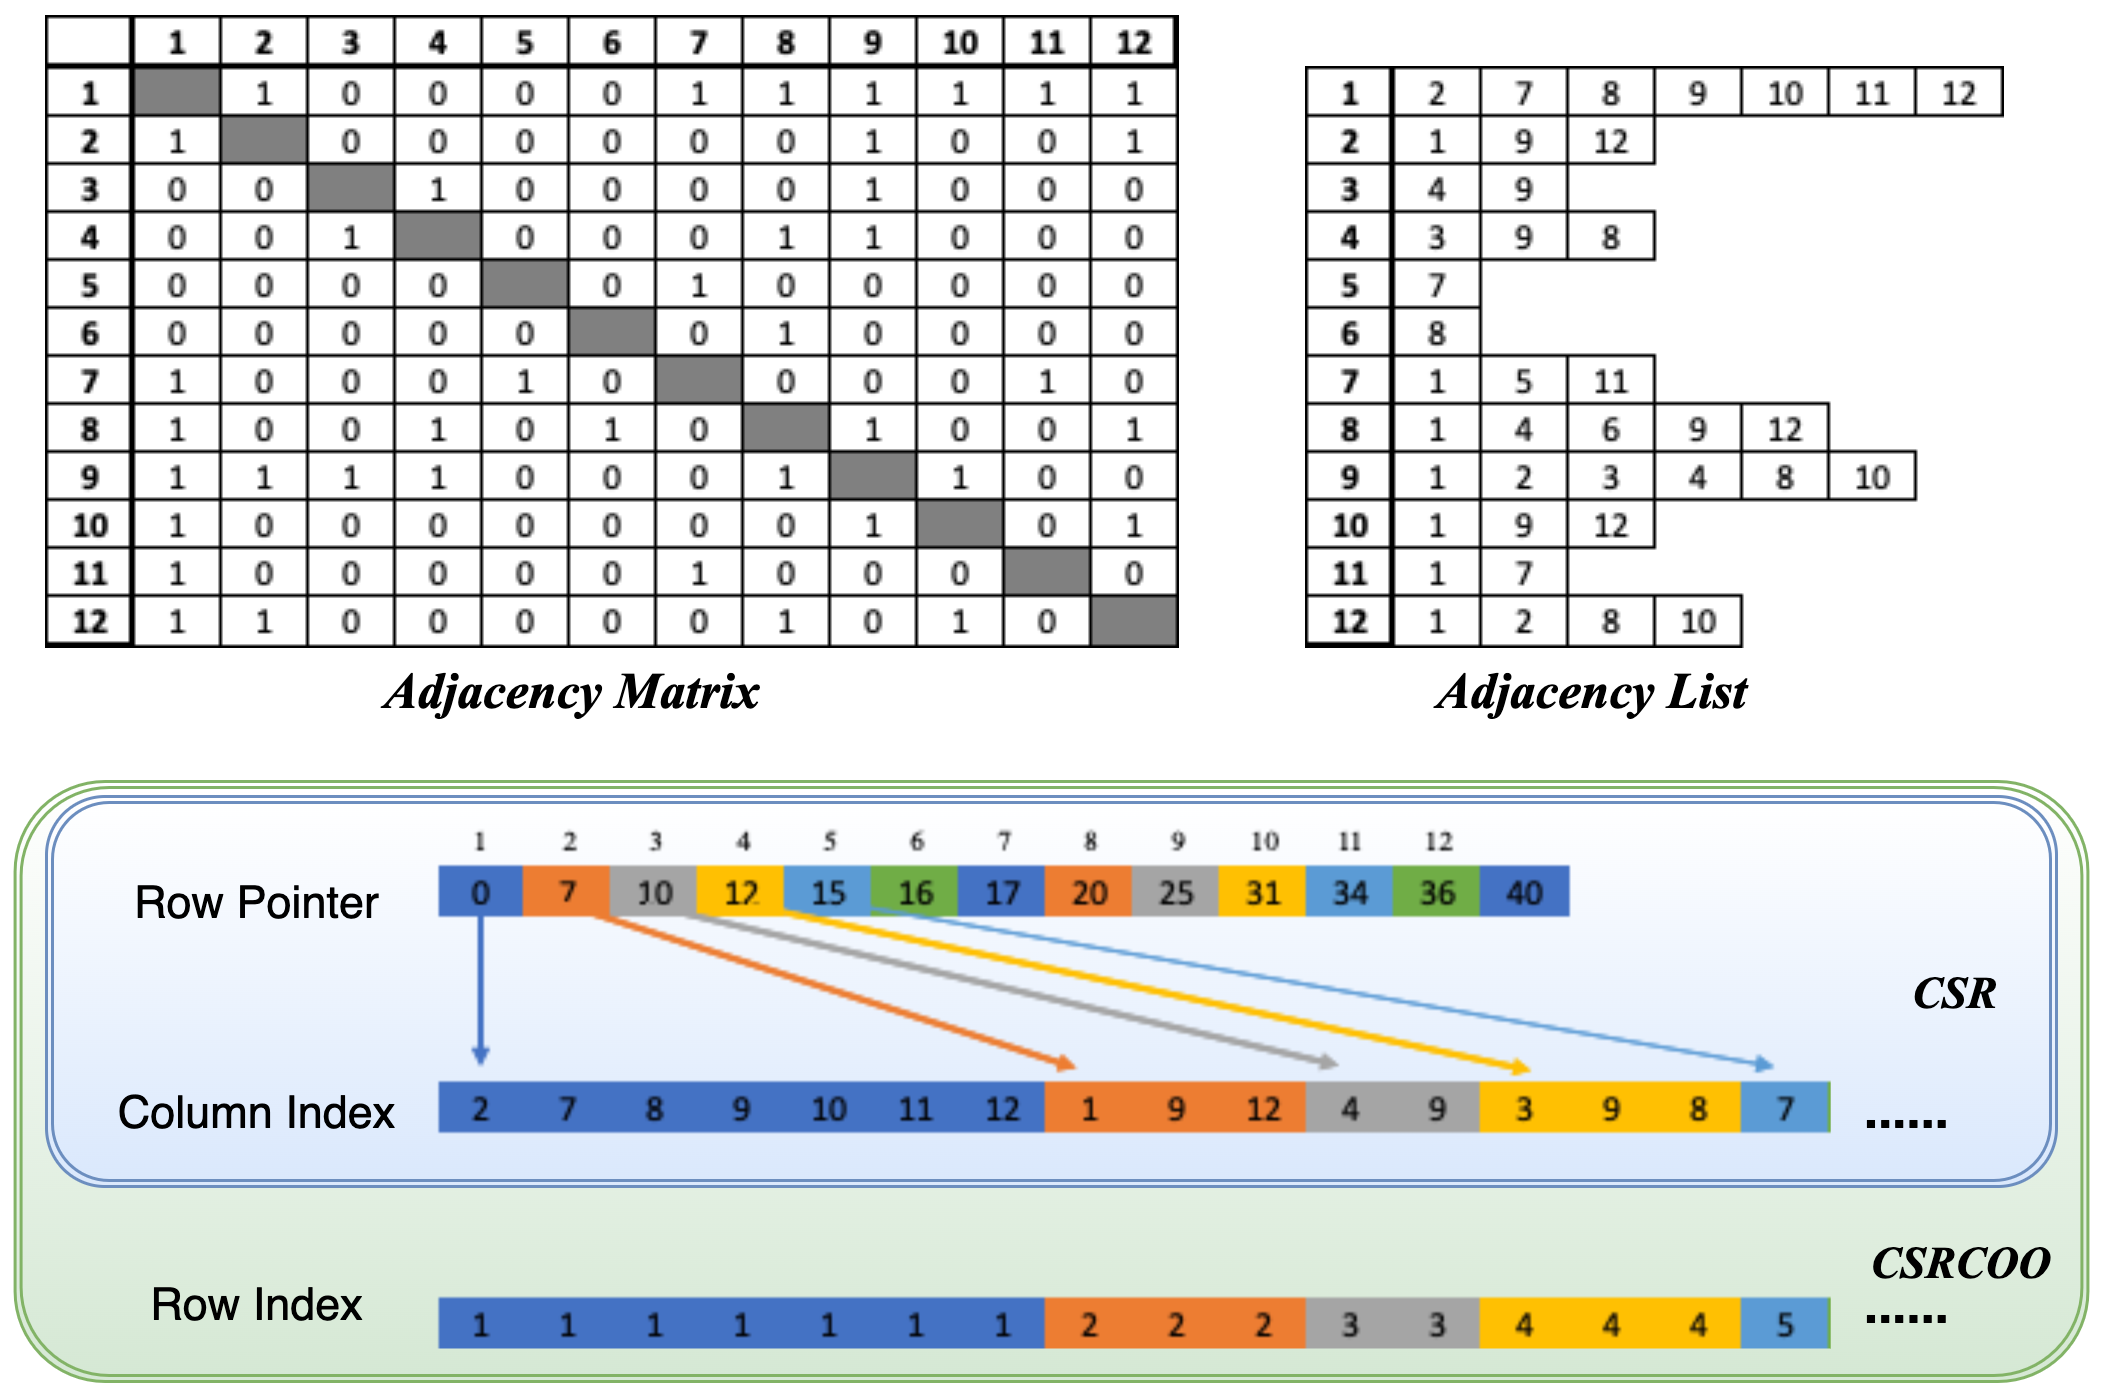
\includegraphics[width=\textwidth]{fig/graph-storage.png}
    \caption{Graph Storage Formats for graph in Fig.\ \ref{fig:sgm-intro}}
    \label{fig:graph-storage}
\end{figure}

We use a combination of CSR and COO formats in our implementation, it is referred as the CSRCOO (Column Sparse Row with COOrdinate) format.
The CSRCOO format uses 3 arrays for storing information of the underlying graph.
These arrays are \textit{Row Pointer} $|V|+1$, \textit{Row Index} $|E|$ and \textit{Column Index} $|E|$
% Here the first 3 arrays are same as the standard CSR and COO arrays, the $4^{th}$ array stores the column indices in a segment wise sorted fashion based on a given rule.
% We use Degree and Degeneracy as 2 rules in this work.
We maintain the \textit{Row Index} and \textit{Column Index} arrays sorted by their labels to enable binary search.
Figure \ref{fig:graph-storage} shows comparison between different graph storage formats.
